\providecommand{\econtexRoot}{}
\renewcommand{\econtexRoot}{..}
% The \commands below are required to allow sharing of the same base code via Github between TeXLive on a local machine and Overleaf (which is a proxy for "a standard distribution of LaTeX").  This is an ugly solution to the requirement that custom LaTeX packages be accessible, and that Overleaf seems to ignore symbolic links (even if they are relative links to valid locations)
\providecommand{\econtex}{\econtexRoot/texmf-local/tex/latex/econtex}
\providecommand{\econtexSetup}{\econtexRoot/texmf-local/tex/latex/econtexSetup}
\providecommand{\econtexShortcuts}{\econtexRoot/texmf-local/tex/latex/econtexShortcuts}
\providecommand{\econtexBibMake}{\econtexRoot/texmf-local/tex/latex/econtexBibMake}
\providecommand{\econtexBibStyle}{\econtexRoot/texmf-local/bibtex/bst/econtex}
\providecommand{\notes}{\econtexRoot/texmf-local/tex/latex/handout}
\providecommand{\handoutSetup}{\econtexRoot/texmf-local/tex/latex/handoutSetup}
\providecommand{\handoutShortcuts}{\econtexRoot/texmf-local/tex/latex/handoutShortcuts}
\providecommand{\handoutBibMake}{\econtexRoot/texmf-local/tex/latex/handoutBibMake}
\providecommand{\handoutBibStyle}{\econtexRoot/texmf-local/bibtex/bst/handout}

  
\providecommand{\EqDir}{\econtexRoot/Equations}
\providecommand{\FigDir}{\econtexRoot/Figures}
\providecommand{\CodeDir}{\econtexRoot/Code}
\providecommand{\DataDir}{\econtexRoot/Data}
\providecommand{\SlideDir}{\econtexRoot/Slides}
\providecommand{\TableDir}{\econtexRoot/Tables}
\providecommand{\ApndxDir}{\econtexRoot/Appendices}

\providecommand{\ResourcesDir}{\econtexRoot/Resources}
\providecommand{\LaTeXFiles}{\econtexRoot/LaTeX}
 
\documentclass[titlepage]{\econtex} 
\usepackage{xr-hyper}
\usepackage{graphicx}
\usepackage{float}
\graphicspath{ {./Pictures/} }
% The \commands below are required to allow sharing of the same base code via Github between TeXLive on a local machine and Overleaf (which is a proxy for "a standard distribution of LaTeX").  This is an ugly solution to the requirement that custom LaTeX packages be accessible, and that Overleaf seems to ignore symbolic links (even if they are relative links to valid locations)
\providecommand{\econtex}{\econtexRoot/texmf-local/tex/latex/econtex}
\providecommand{\econtexSetup}{\econtexRoot/texmf-local/tex/latex/econtexSetup}
\providecommand{\econtexShortcuts}{\econtexRoot/texmf-local/tex/latex/econtexShortcuts}
\providecommand{\econtexBibMake}{\econtexRoot/texmf-local/tex/latex/econtexBibMake}
\providecommand{\econtexBibStyle}{\econtexRoot/texmf-local/bibtex/bst/econtex}
\providecommand{\notes}{\econtexRoot/texmf-local/tex/latex/handout}
\providecommand{\handoutSetup}{\econtexRoot/texmf-local/tex/latex/handoutSetup}
\providecommand{\handoutShortcuts}{\econtexRoot/texmf-local/tex/latex/handoutShortcuts}
\providecommand{\handoutBibMake}{\econtexRoot/texmf-local/tex/latex/handoutBibMake}
\providecommand{\handoutBibStyle}{\econtexRoot/texmf-local/bibtex/bst/handout}

  
\providecommand{\EqDir}{\econtexRoot/Equations}
\providecommand{\FigDir}{\econtexRoot/Figures}
\providecommand{\CodeDir}{\econtexRoot/Code}
\providecommand{\DataDir}{\econtexRoot/Data}
\providecommand{\SlideDir}{\econtexRoot/Slides}
\providecommand{\TableDir}{\econtexRoot/Tables}
\providecommand{\ApndxDir}{\econtexRoot/Appendices}

\providecommand{\ResourcesDir}{\econtexRoot/Resources}
\providecommand{\LaTeXFiles}{\econtexRoot/LaTeX}


% \owner determines where links to online content go
% llorracc is Chris Carroll's personal version
% econ-ark is the Econ-ARK/REMARK version
%\providecommand{\owner}{llorracc}
\providecommand{\owner}{econ-ark}


\providecommand{\texname}{OptimalTaxHeight}
\usepackage{\LaTeXFiles/BufferStockTheory}

\begin{document}

\providecommand{\versn}{}
\ifthenelse{\boolean{ifWeb}}{  \renewcommand{\ushort}{\underline}\renewcommand{\versn}{Web} }{} 

\hfill{\tiny \jobname~\versn~\today~{at} \DTMcurrenttime, \input{\ResourcesDir/.git-source-commit}~~\input{\ResourcesDir/.git-public-commit}}

\title{The Optimal Taxation of Height: \\ A Case Study of Utilitarian Income Redistribution}

\author{N. Gregory Mankiw and Matthew Weinzierl \\ Ballpark by: Muhammad Syareza Lumban Tobing\authNum}

\keywords{Optimal Taxation}

\jelclass{D64, H21, H23, H24, J11\\
  \href{https://econ-ark.org}{
\includegraphics{\ResourcesDir/PoweredByEconARK}}
}

\renewcommand{\forcedate}{October 16, 2020}
\date{\forcedate}

\maketitle 
\hypertarget{abstract}{}
\begin{abstract}
 The authors apply a standard utilitarian framework to analyze whether policy makers should include height as a ''tag'' when designing the income tax system. In order to measure the gains from incorporating height, they calculate the windfall that a planner with a bencmark tax design which does not include height, would have to gain to be able to receive the same aggregate welfare as a planner that does take height into account. By running a simulation based on a sample of fully-employed white males in 1996, they found that a tall person earning \$50,000 should pay \$4,500 more in tax compared to a short person.
\end{abstract}

\begin{authorsinfo}
  \name{Contact: \href{mailto:}{\texttt{mtobing1@jhu.edu}}, Department of Economics, Wyman Hall, Johns Hopkins University, Baltimore, MD 21218, \url{https://github.com/raytobing}}
\end{authorsinfo}

\newcommand{\thankstext}{Thank you to Prof. Christopher D. Carroll for the template on which this paper is written.}

\ifthenelse{\boolean{ifWeb}}{}{\thanks{\thankstext}}

\titlepagefinish

\ifthenelse{\boolean{ifWeb}}{\medskip \noindent {\tiny
    \thankstext \medskip \medskip \medskip
  }}{\pagebreak 
}

\ifthenelse{\boolean{ifWeb}}{\medskip \noindent {\footnotesize \thankstext} \\  {\centering \medskip \medskip \medskip  \noindent \hrule height 0.4pt depth 0.0pt width \textwidth \relax}}{\pagebreak } % \end{Web}

\hrule height 0.4pt depth 0.0pt width \textwidth \relax

\medskip \medskip

\hypertarget{Overview}{}
\section{Overview}

A utilitarian social planner that would like to transfer resources from high-ability to low-ability individuals is generally constrained by their inability directly observe ability.

If the planner is allowed to use other exogenous variables such as  height that is proven to be correlated with ability in designing their tax policies, it would be in their benefit to do so.
Consequently, in order to show the benefits of incorporating taxation into the income tax design, the authors ran a number of simulations based on actual data using a sample of white males in their thirties from 1996 to which they found that incorporating  height as a tag in taxing income would cause an increase in the average tax rate faced by tall people while at the same time resulting in shorter individuals receiving income transfers. The simulations also estimates the annual income, consumption, labor supply and utility obtained by each height group given a simulated tax policy.  At the same time, by using a benchmark model in which height is not incorporated into the tax design, the authors shows that incorporating height allows a  utilitarian social planner to  yield a modest annual welfare gain for the economy.

There are a number of simulations done by the author in this paper, including:
\begin{itemize}
  \item Optimal taxes under the benchmark model where the planner ignores height 
  \item Optimal taxes where the planner incorporates height
  \item Optimal taxes including height with varying risk aversion
  \item Optimal taxes including height with varying labor supply elasticity
\end{itemize}

\hypertarget{The Model}{}
\section{The Model}

\hypertarget{General Framework}{}
\subsection{General Framework}

The population is dividied into $H$ height groups that are indexed by $\h$ and population proportions $p_h$. In each height group, each person has wages that can take one of $I$ possible values. The wage distribution in each height group is given by $\pi_h = \{ \pi_{h,i}\}_{i=1}^I$ meaning that the proportion $\pi_{h,i}$ of each height group $h$ has wage $w_i$.

On the other hand, individual income $y_{h,i}$ is the product of labor effort $l_{h,i}$ and wage, given by:

\begin{align}
    y_{h,i} \ = \ w_i l_{h,i}. 
\end{align}

  We assume that both labor effort and wage are private information, with only height and income being transparent to the government.

  Subsequently, the individual utility function is set as a function of consumption (increasing and concave) and labor effort (decreasing and convex). Consumption is set to be equal to after-tax income and taxes can be a function of income and height.

  The objective of the social planner is to  maximize a utilitarian social welfare function by choosing a bundle of consumption and income. The planner is met with the constraint that taxes are purely redistributive (it does not fund government expenditure) and by what they can observe. This leads to the application of the Revelation Principle, where the policy design will induce each individual to reveal their true wage and effort level when choosing their bundles.

  Consequently, the social planners maximization problem can be stated as:
 \begin{align}
   \max_{c,y}~ \sum_{i=1}^I \ p_{h} \sum_{i=1}^I \ \pi_{h,i} u\left(c_{h,i}, \frac{y_{h,i}}{w_i}\right)
 \end{align}
 The maximization problem is subject to the following individual incentive compatibility constraints:
 \begin{align}
   u\left(c_{h,i}, \frac{y_{h,i}}{w_i}\right) \geq u\left(c_{h,j}, \frac{y_{h,j}}{w_j}\right)
 \end{align}
 for all $j$ for each individual with height $h$ and wage $w_i$, where $c_{h,j}$ and $y_{h,j}$ are the allocations intended to be chosen by the planner with the aforementioned height and wage.

 The planner's problem as stated above can be separated into two separate problems, namely, setting optimal taxes within height groups and setting optimal aggregate transfers between height groups. If we let $\{R_h\}_{h=1}^H$ be the transfer paid by each group h, the planner's problem then becomes:

  \begin{align}
   \max_{\{c,y,R\}}~ \sum_{i=1}^I \ p_{h} \sum_{i=1}^I \ \pi_{h,i} u\left(c_{h,i}, \frac{y_{h,i}}{w_i}\right)
 \end{align}
 This problem is subject to H height-specific feasibility constraints:

   \begin{align}
    \sum_{i=1}^I \ \pi_{h,i} \ (y_{h,i} - c_{h,i}) \geq R_h ;
 \end{align}
 given this equation, let the multipliers on the H conditions given by equation (5) be $\{\lambda_h\}_{h=1}^H$.

 By using the two-part approach, when the first-order condition with respect to $R_h$ is calculated, we then obtain the following optimality condition:

   \begin{align}
    \lambda_h \ = \ \lambda_{h'}
   \end{align} 
   which applies for all the height groups, $h$ and $h'$, meaning that the marginal social cost of increasing the tax revenue is equal across the different types.

   Besides the previous model, the authors also consdier a ``benchmark'' model, in which a planner does not use height in the design of their income tax system. The benchmark model is captured by the following inequality:

    \begin{align}
     u\left(c_{h,i}, \frac{y_{h,i}}{w_i}\right) \geq u\left(c_{g,j}, \frac{y_{g,j}}{w_i}\right)
    \end{align}

    The benchmark model will be used to measure the gain from including weight in the design of the income tax system, which will be done by calculating the windfall the social planner would have to obtain to be able to achieve the same aggregate welfare as an optimal planned who incoporates height into their tax design.
 
\hypertarget{Analytical Result}{}
\subsection{Analytical Result}

In the analytical analysis, utility is assumed to be additively separable between consumption and labor, exhibits constant relative risk aversion (CRRA) in consumption and is isoelastic in labor:

   \begin{align}
  u\left((c_{h,i}), \frac{y_{h,i}}{w_i}\right) \ = \ \frac{(c_{h,i}^{1-\gamma}) \ - \ 1}{1 \ - \ \gamma} - \frac{\alpha}{\sigma} \left(\frac{y_{h,i}}{w_i}\right)^\sigma.
   \end{align}
$\gamma$ determines the concavity of utility from consumption,  $\alpha$ is the relative wieght of consumption and leisure in the utility function and $\sigma$ is the elasticity of labor supply. In particular, the authors are interested in $\frac{1}{(\sigma \ - \ 1)}$, which is the compensated (constant-consumption) labor supply elasticity.

By applying the two-part method in the previous section, we can rewrite the planner's problem as:

\begin{align}
\max_{\{c,y,R\}} \ \sum_{i=1}^I \ p_{h} \sum_{i=1}^I \ \pi_{h,i} \left[ \frac{(c_{h,i})^{1-\gamma} \ - \ 1}{1 \ - \ \gamma} - \frac{\alpha}{\sigma} \left(\frac{y_{h,i}}{w_i}\right)^\sigma \right];
\end{align}  
that is subject to H feasibility constraints definded below:
\begin{align}
    \sum_{i=1}^I \ \pi_{h,i} \ (y_{h,i} - c_{h,i}) \geq R_h ;
 \end{align}
 along with an incentive constraint for each indvidual:
 \begin{align}
   \frac{(c_{h,i})^{1-\gamma} \ - \ 1}{1 \ - \ \gamma} \ - \  \frac{\alpha}{\sigma} \left(\frac{y_{h,i}}{w_i}\right)^\sigma \geq \frac{(c_{h,j})^{1-\gamma} \ - \ 1}{1 \ - \ \gamma} \ - \  \frac{\alpha}{\sigma} \left(\frac{y_{h,j}}{w_i}\right)^\sigma
\end{align}

From the analytical result, we can obtain two characteristics of the optimal height tax.

First, the first-order condition for consumption and income imply that no marginal taxation of the top earner holds for the top earners in all height groups. This means that optimal allocations satisfies the following equation:
\begin{align}
  (c_{h,I})^{- \gamma}= \frac{\alpha}{w_I}\left( \frac{y_{h,I}}{w_l}\right)^{\sigma - 1}
  \end{align}

  Second, the average cost of increasing social welfare is equalized across height groups as captured by the following equation:
\begin{align}
  \sum_{i=1}^I \pi_{h,i} (c_{h,i})^\gamma =  \sum_{i=1}^I \pi_{g,i} (c_{g,i})^\gamma
  \end{align}
  for all height groups $g,h$. The term $(c_{h,i})^\gamma$ is the cost, in unit of consumption, of a marginal increase in the uitlity of individual $h, \ i$.

\hypertarget{Data}{}
\section{Data}

The authors uses data from the National Longitudinal Survey of Youth (NLSY) and focuses only on adult white males. The data is limited to men aged between 32 and 39 in 1996 that were working at least 1,000 hours that year, which nets the final sample to 1,738 observations.

\begin{table}[H]
  \centering
    \caption{Height Distribution of Adult White Male Full-Time Workers in The United States}
    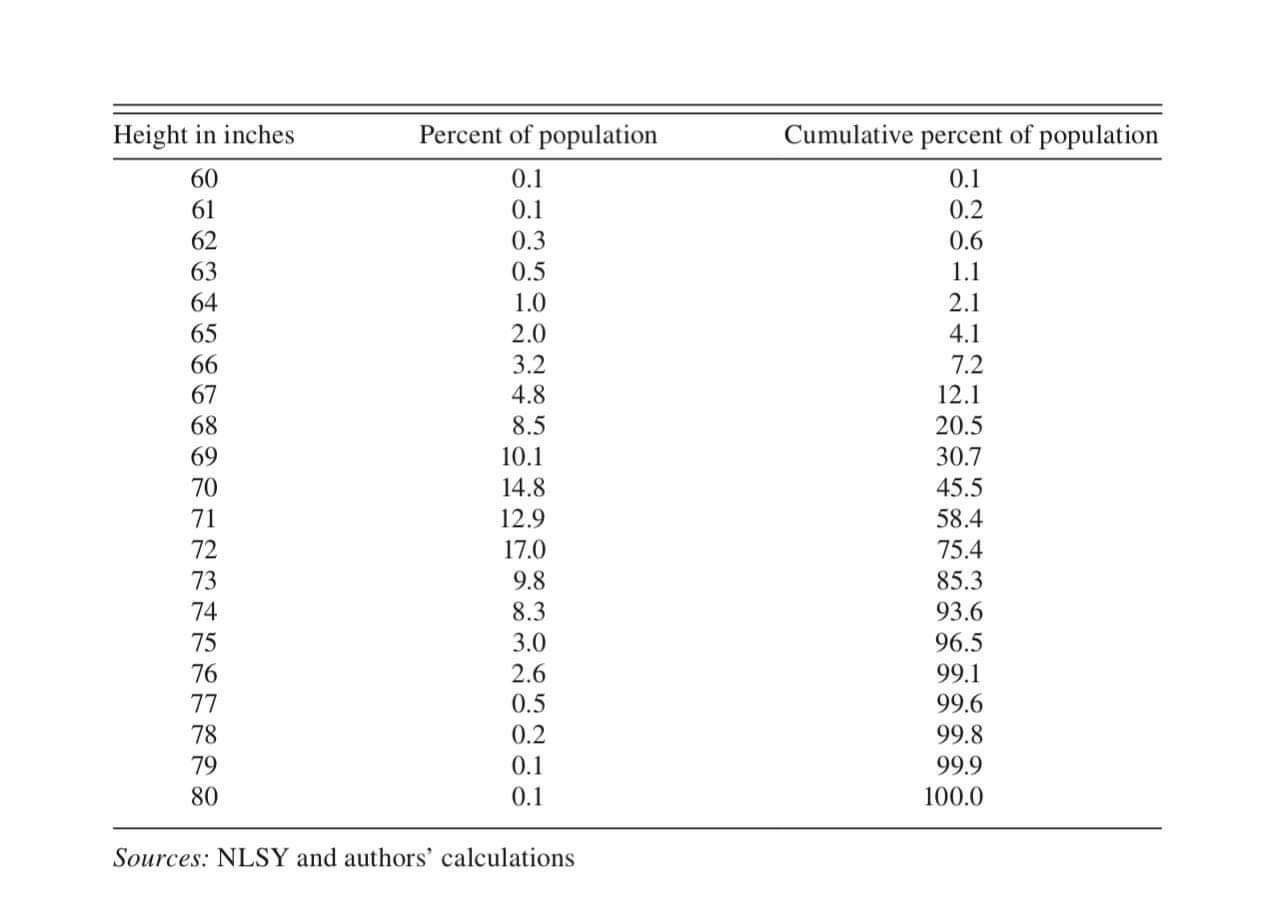
\includegraphics[width=0.8\textwidth]{HeightDistribution.JPG}
    \label{fig:Table 1}
  \end{table}
  
  Table \ref{fig:Table 1} shows the distribution, by height of the sample used. The population is split into three groups: ``tall'' which are men that are taller than 72 inches, ``medium'' for men  between 70 and 72 inches and ``short'' for those who are below 70 inches tall .
  
\begin{figure}[H]
  \centering
  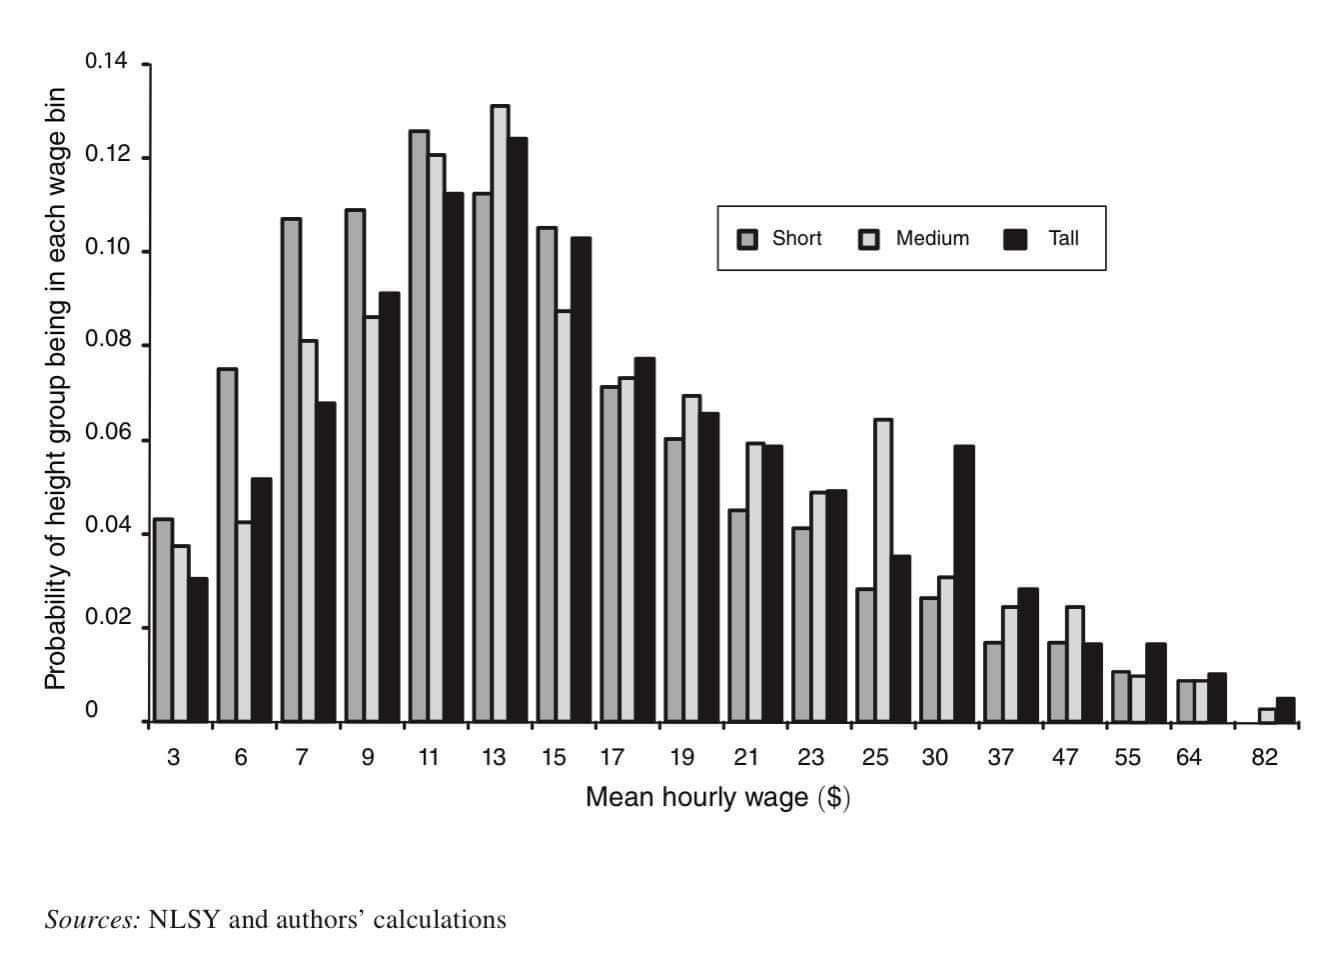
\includegraphics[width=1\textwidth, height=10cm]{WageDistributionGraph.JPG}
  \caption{Wage Distribution of Adult White Males in The United States by Height}
    \label{fig:Figure 1}
  \end{figure}

  As shown in Figure \ref{fig:Figure 1}, the distribution of wages for the tall group has a higher mean wage compared to the short group. The distribution are similar around the most common wages but different towards the tails. The tall group has an average wage that is 16 percent higher compared to the short group suggesting that an inch of height adds just over 2 percent to wages.

\hypertarget{Simulation Results}{}
\section{Simulation Results}

In simulating the model, the utility function shown at the beginning of section 2.2 is used:
   \begin{align}
  u\left((c_{h,i}), \frac{y_{h,i}}{w_i}\right) \ = \ \frac{(c_{h,i})^{1-\gamma} \ - \ 1}{1 \ - \ \gamma} - \frac{\alpha}{\sigma} \left(\frac{y_{h,i}}{w_i}\right)^\sigma
   \end{align}
   where $\gamma$ is the curvature of the utility of consumption, $\alpha$ is a taste parameter and $\sigma$ is the compensated (constant-consumption) elasticity of labor supply that is equal to $\frac{1}{\sigma \ - \ 1}$. The baseline values used for the parameters are $\gamma = 1.5$, $\alpha = 2.55$ and $ \sigma = 3$. As a comparison, the authors have also calculated optimal taxes under the benchmark model specified in the previous section.

\begin{figure}[H]
  \centering
  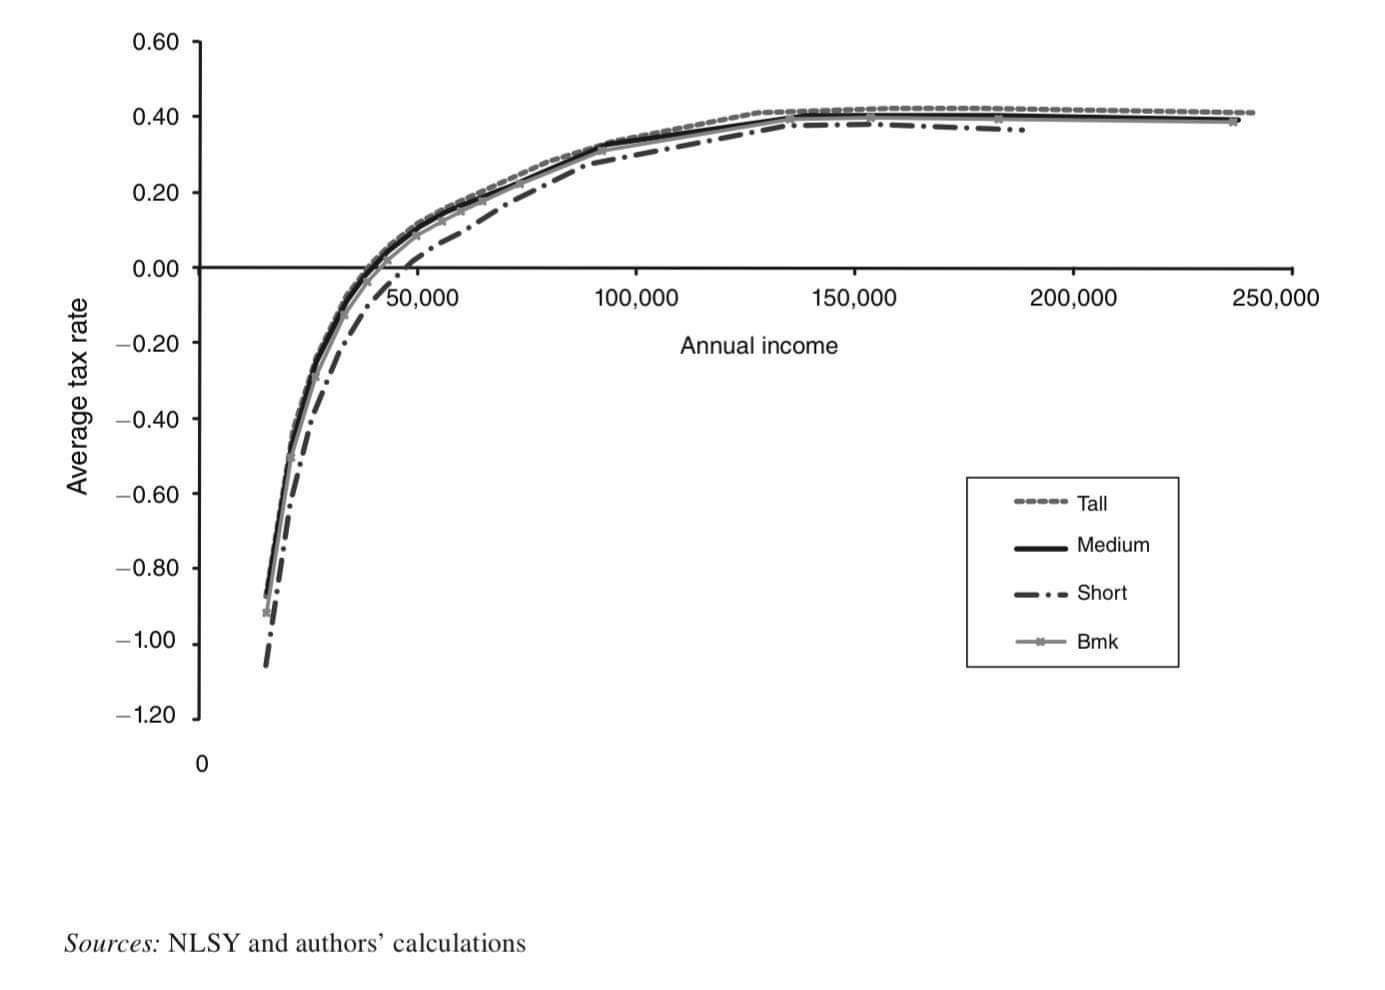
\includegraphics[width=1\textwidth, height=12cm]{AverageTax.JPG}
  \caption{Average Tax Rates}
    \label{fig:Figure 2}
  \end{figure}
   
  Figure \ref{fig:Figure 2} exhibits the average tax rate schedules for the all three height groups in the optimal model along with the average tax rate obtained from the benchmark model. If we observe the relative positions of the average tax sschedules in Figure  \ref{fig:Figure 2}, we can see that the average tax rate of short individuals is always below tall individuals, with the gap caused by the lump-sum transfer between groups. It can be concluded that the optimal average tax rate increases quickly at low-income levels and then tapers off as income increases. 

\begin{figure}[H]
  \centering
  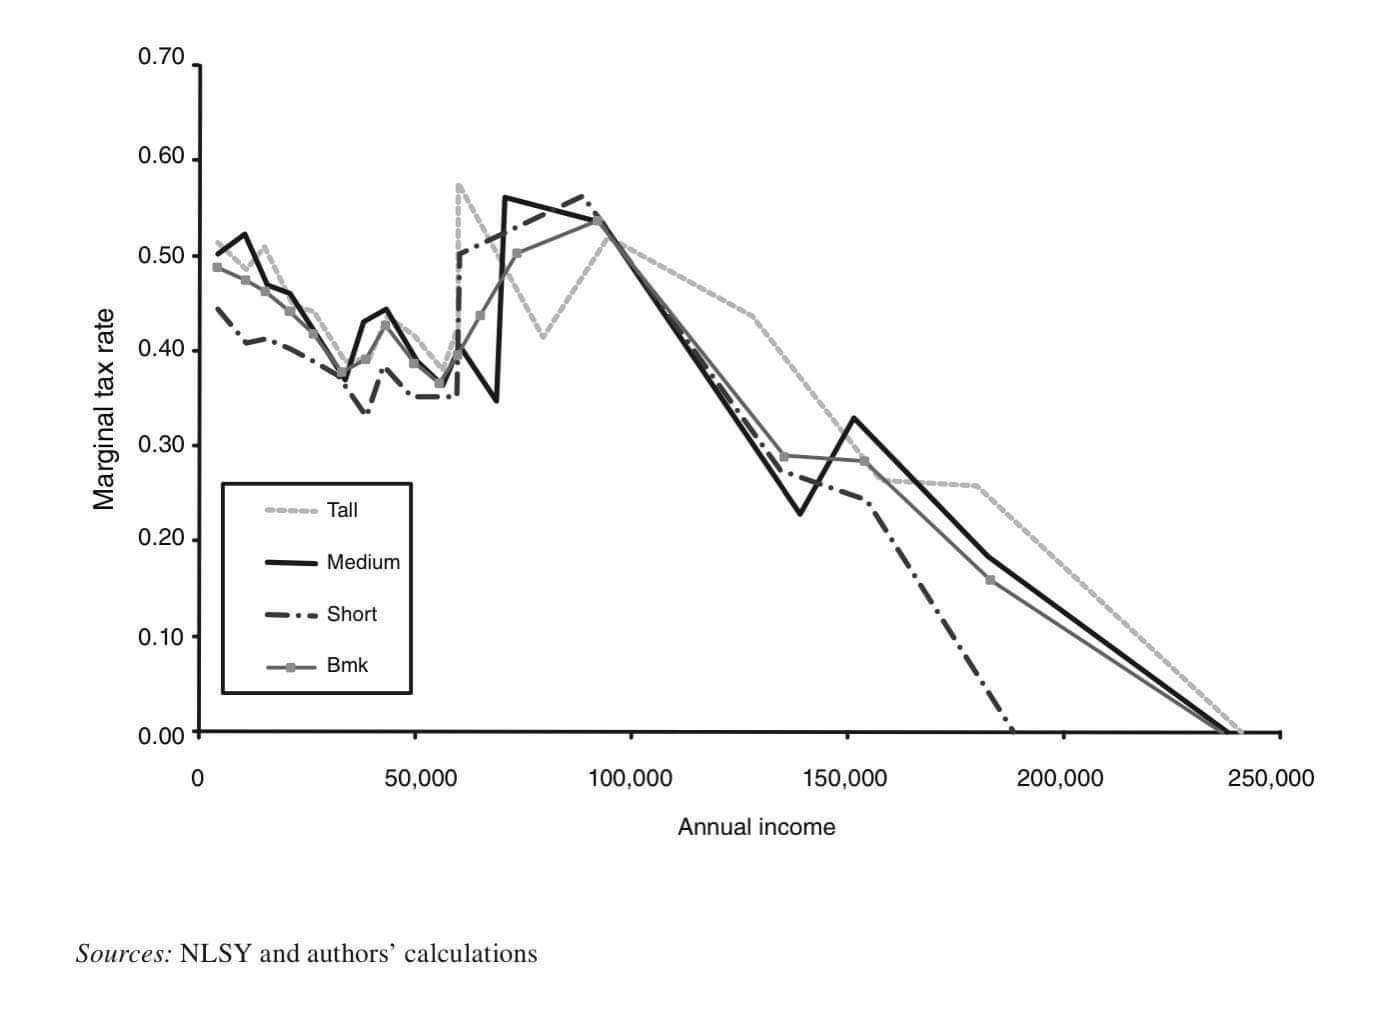
\includegraphics[width=1\textwidth, height=12cm]{MarginalTax.JPG}
  \caption{Marginal Tax Rates}
    \label{fig:Figure 3}
  \end{figure} 

  Subsequently, Figure \ref{fig:Figure 3} shows the marginal tax rate schedules, which is calculated as the implicit wedge that the optimal allocation inserts into the individual's private equilibrium consumption-leisure tradeoff. We can see from the figure that the marginal tax rate is approximately flat for most incomes followed by a sharp drop to zero for the highest earners in each group.

  Using the assummed functional formes, the first order conditions for consumption and leisure implies that the marginal tax rate can be calculated as:
\begin{align}
  T'(y_{h,i}, \ h) \ = \ 1 \ + \ \frac{u_y(c_{h,i}, \ \frac{y_{h,i}}{W_i})}{u_c(c_{h,i}, \ \frac{y_{h,i}}{W_i}}) \ = \ 1 \ - \ \frac{\alpha(\frac{y_{h,i}}{W_i})^{\sigma-1}}{w_i(c_{h,i})^{-\gamma}},
\end{align}
where $T'(y_{h,i}, \ h)$ is the height specific marginal tax rate at the income level $y_{h,i}$.
  

\begin{table}[H]
  \centering
  \label{fig:Table 2}
  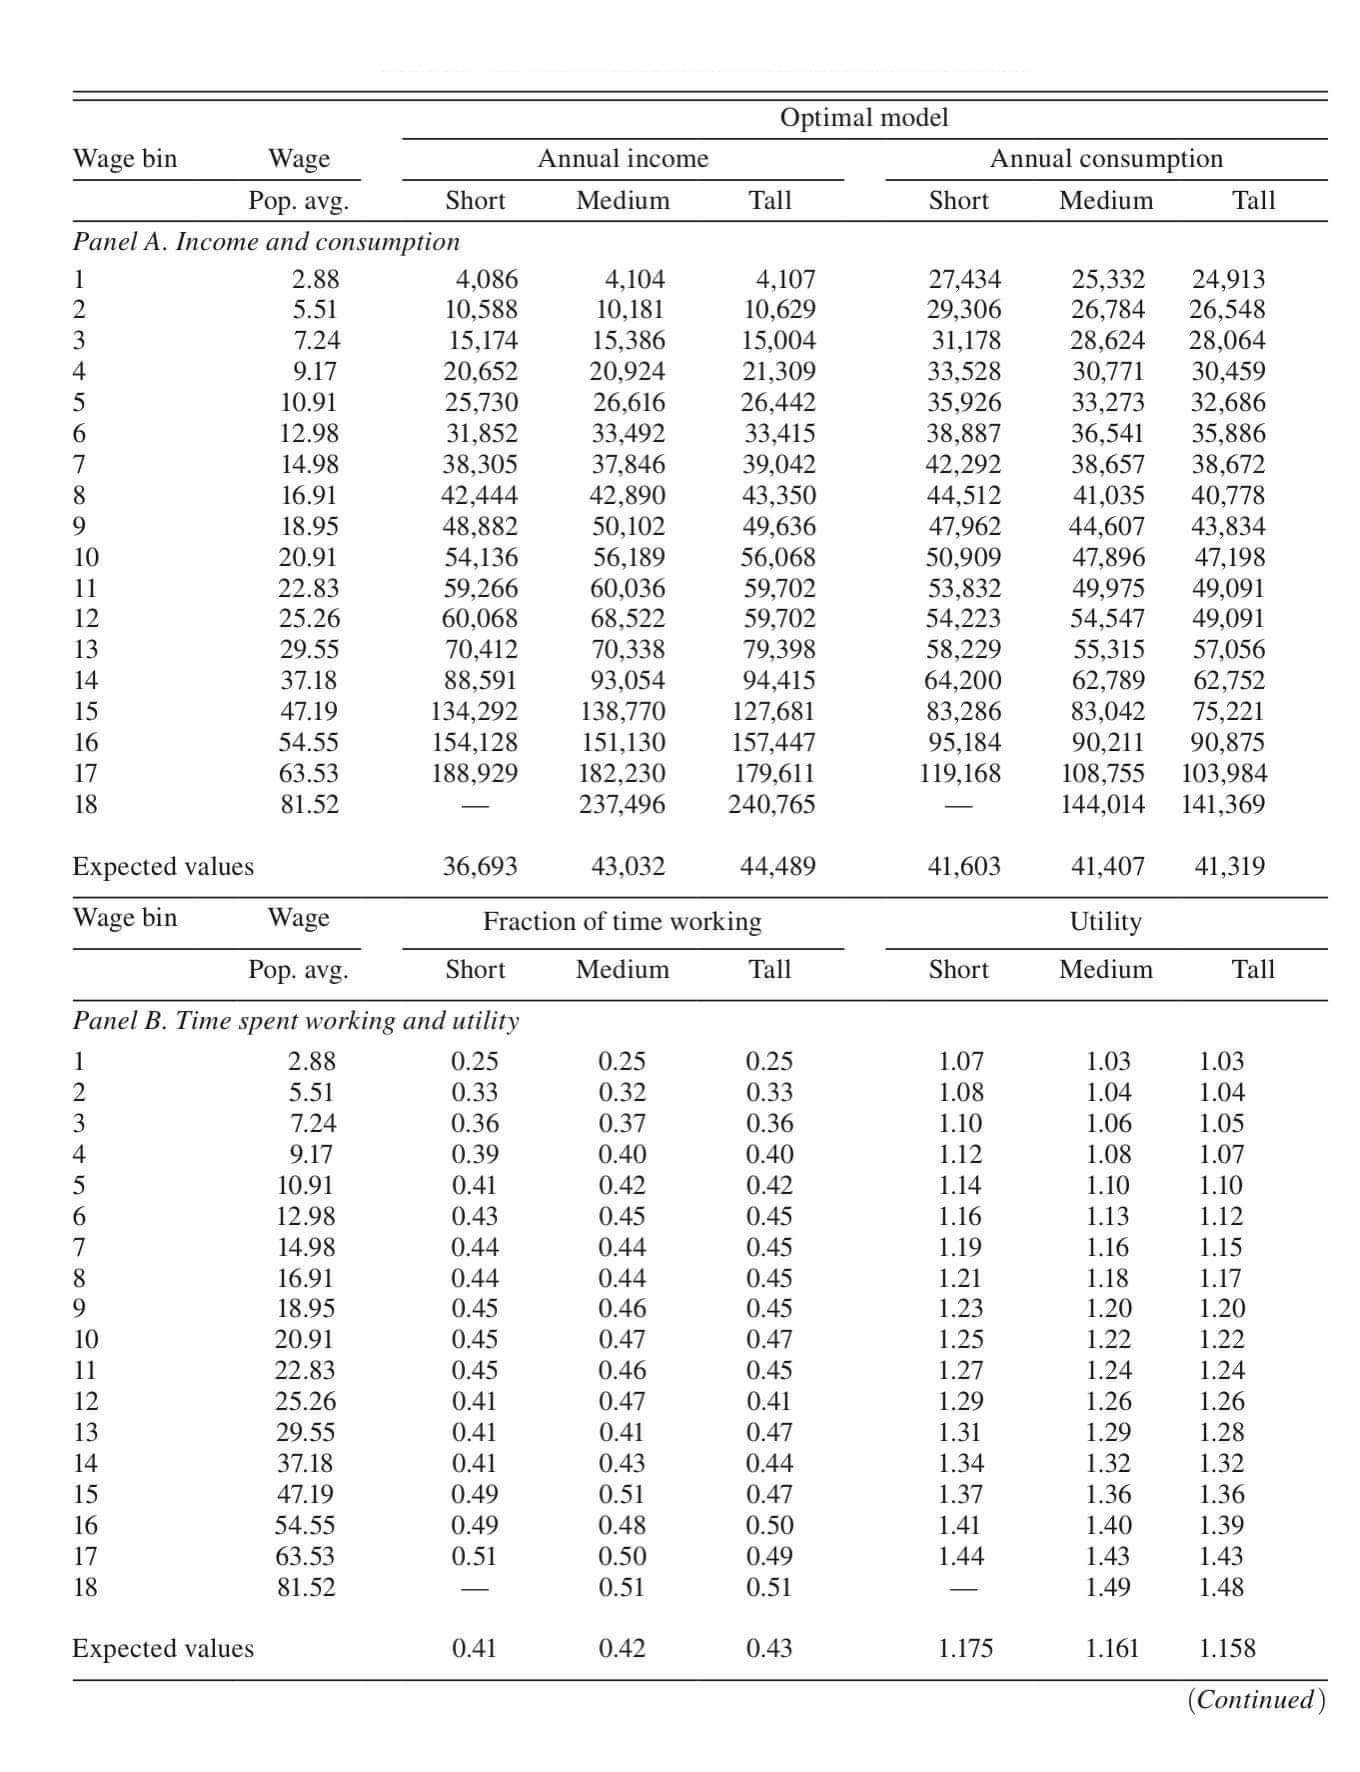
\includegraphics[width=0.8\textwidth]{OptimalAllocationBaseline1.JPG}
  \caption{Marginal Tax Rates}
  \end{table}


  Table 2 and Table 3 lists the income, consumption, labor and utility levels as well as tax paymernts, average tax rates and marginal tax rates at each wage level for the height groups in the optimal model. From the two tables, we can see that the average tax on the tall group is around 7.1 percent of their average income, while the short group receives a transfer of more than 13 percent of their income.

\begin{table}[H]
  \centering
  \label{fig:Table 3}
  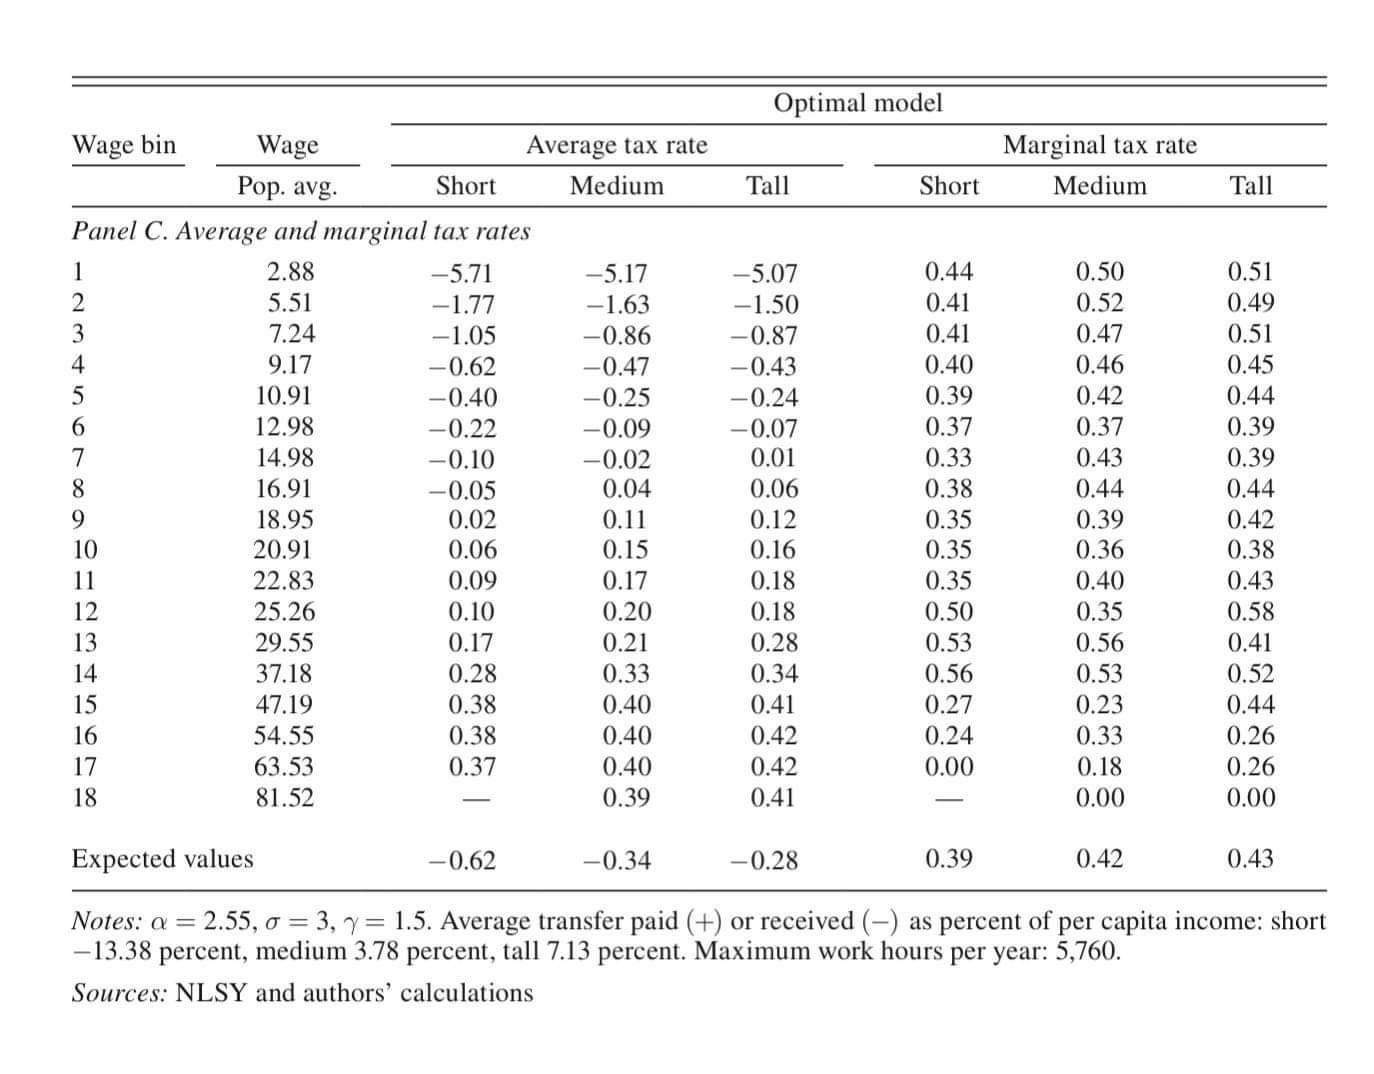
\includegraphics[width=0.8\textwidth]{OptimalAllocationBaseline2.JPG}
  \caption{Marginal Tax Rates (Continued)}
  \end{table}  
  Table 3 also shows that when height is included in the tax design, the tall group of individuals receive smaller utility for a given wage compared to the other two groups, which results in a lower expected utility for the tall group as a whole compared to the two shorter groups. This finding coincides with the result of optimal tax theory when ability can be observed by the policy makers

Using the results from Table 2 and Table 3, the authors also created a tax schedule that resembles used by US taxpayers with results shown in Table \ref{fig:Table 4}.
  
\begin{table}[H]
  \centering
  \label{fig:Table 4}
  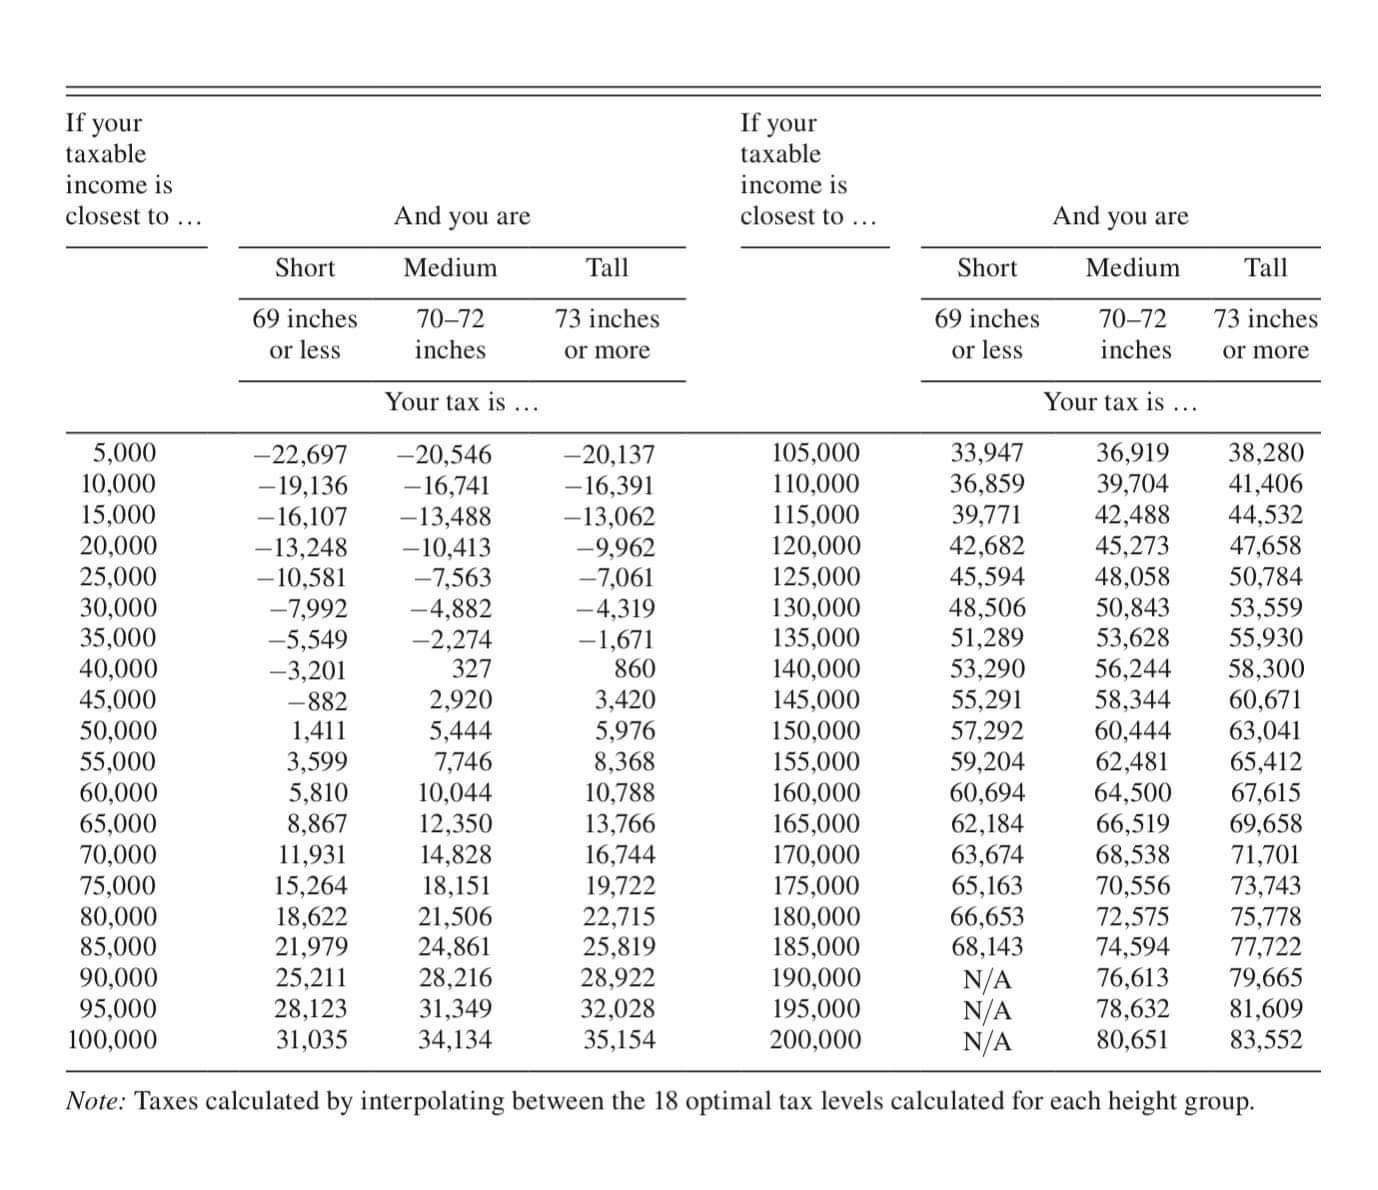
\includegraphics[width=0.8\textwidth]{ExampleTaxTable.JPG}
  \caption{Example Tax Table}
  \end{table}  

  In the actual US tax schedule, tax payers generally look across columns of family status in order to determine how much tax credit they would be able to receive. On the other hand, the tax schedule created in Table 4 has height groups across the columns, which determines the amount of tax an individual must pay given their income or the amount of transfers they are eligible to receive given their wage group.

 From Table \ref{fig:Table 4}, we can see that the tall group pays more taxes compared to the short group for most income levels. For example, a tall person with \$50,000 pays \$4,500 more in taxes than a short person earning the same amount of pre-tax income. Transfers stop for the short group once their income hits \$50,000. Also notice that the short group would not pay any income tax when after their income rises above \$190,000.

\begin{table}[H]
  \centering
  \label{fig:Table 5}
  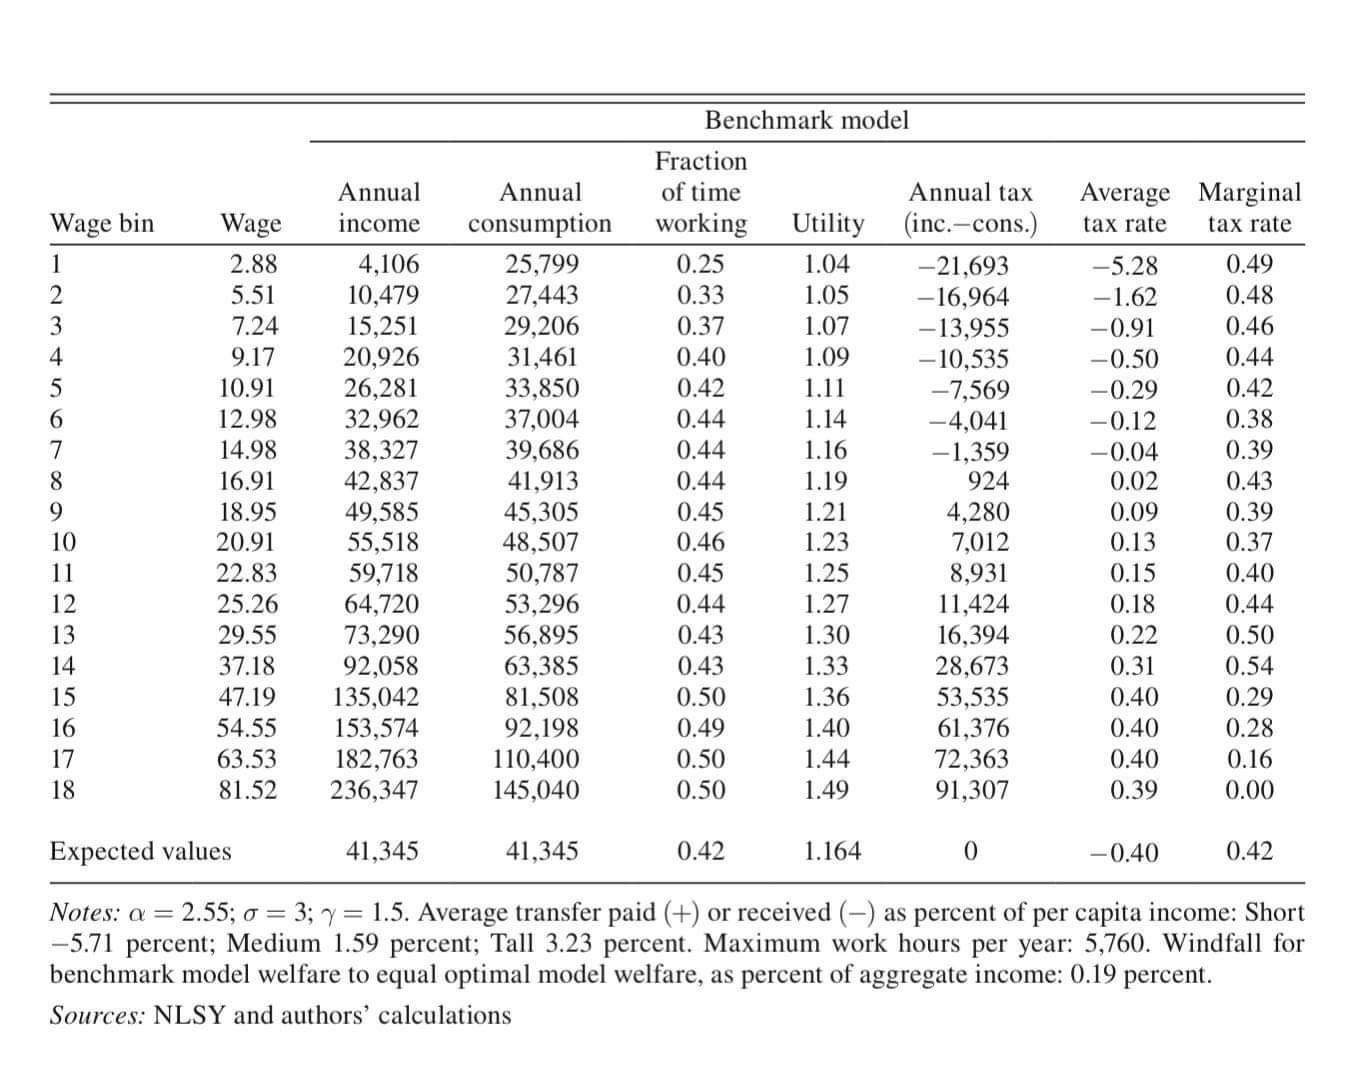
\includegraphics[width=0.8\textwidth]{BenchmarkCase.JPG}
  \caption{Benchmark Case}
  \end{table}
  
  Finally, the authors uses the benchmark model to create Table 5 in which they calculate a money-metric welfare gain from the height tax by finding the windfall revenue that allows the benchmark planner to reach the same level of welfare as the optimal planner that tags height. The table shows that the required windfall is around 0.19 percent of aggregate income meaning that given a hypothetical GDP of \$12 trillion, a height tax yields an annual welfare gain of about \$24 billion.

\hypertarget{Conclusions}{}
\section{Conclusions}

This paper is essentially a thought exercise generated by the authors to start a discussion on the central assumption of the standard approach to the optimal design of tax policy.

By conducting a simulation based on a sample of white male obtained from the  NLSY collected in 1996, the author found that by incorporating height into the income tax design, a utilitarian social planner is able to yield an annual welfare gain of \$24 billion in a \$12.5 trillion dollar economy.

\clearpage\vfill\eject

\onlyinsubfile{\bibliography{\econtexRoot/LaTeX/BufferStockTheory,economics}}

\end{document}

